% Preamble: Declarations & Initializations
% DEFINING DOCUMENT CLASS
\documentclass[a4paper, english]{article}

% USING PACKAGES
\usepackage[utf8]{inputenc}
\usepackage{csquotes}
\usepackage[backend=biber,sortcites]{biblatex}
\usepackage{Assets/DUO/duomasterforside}
\usepackage[dvipsnames]{xcolor} % for å kunne et større nummer fargemodeller i en mer fleksibel pakke
\usepackage{amsmath} % for equation*-environmentet
\usepackage{subcaption} % for subfigure-environmentet


% Considering to use:
	% \usepackage[big]{titlesec} % to customize chapters, sections, and sub-sections style in an easy way — https://www.overleaf.com/learn/latex/Sections_and_chapters
	% \usepackage{sectsty} % to customize sections, sub-sections, paragraphs, and sub-paragraphs

% Previously looked at but not found useful yet:
	% \usepackage{sidecap} % for juxtapositioning minipages next to each-other horizontally
	% \usepackage{scalerel} % for scaling objects according to references

% SETTING NEW COMMANDS AND FUNCTIONS
% Text-editing
\newcommand{\tit}[1]{\textit{#1}}
\newcommand{\tbf}[1]{\textbf{#1}}

% Colors
\newcommand{\tcol}[2][red]{\textcolor{#1}{#2}} % default-color is red

% Page-Spacing, -Margins, and -Padding
\newcommand{\nl}{\newline}
\newcommand{\np}{\newpage}

% Lists
\newcommand{\subdash}[1]{\begin{itemize} \item{#1} \end{itemize}}

% ADDING BIBLIOGRAPHY REFERENCE-DATABASE
\addbibresource{Assets/Bibliography/reference_database.bib}

% SETTING PAGE (CONFIGURATION-) PARAMETERS
% Headlines and Titles
\sectionfont{\fontsize{28}{34}\selectfont} % using package 'sectsty'. \fontsize{size}{baselineskip}\selectfont, where baselineskip is approx. 1.2x the size.
	
	% History Archive:
	
	% TRY 1
	% \titleformat*{\section}{\LARGE\bfseries}
	% \titleformat*{\subsection}{\large\bfseries}
	% \titleformat*{\subsubsection}{\large\bfseries}
	% \titleformat*{\paragraph}{\large\bfseries}
	% \titleformat*{\subparagraph}{\large\bfseries}
	
	% TRY 2
	% {\normalfont\Large\bfseries}{\thesection}{1em}{}
	
	% TRY 3
	% \titleformat{\section}{\normalfont\HUGE\bfseries}{\thesection}{1em}{} % using package 'titlesec'
	% \sectionfont{\LARGE} % using package 'sectsty'

% The Document
\begin{document}
	% Dummy-hack chapters to get correct Chapter-numbers: (COMMENT OUT WHEN NECESSARY)
	\chapter{dummy-hack Introduction}
	\chapter{dummy-hack Background}
	\chapter{Baseline}
		\section{Phase-synchronization}
		\section{Phase- \& frequency-synchronization}
		\section{K. Nymoen's bi-directional phase-adjustment}
		\section{K. Nymoen's middle SA-leveled frequency-adjustment}
		\section{System target state: harmonic synchrony}
		\label{sec:harmonic_synchrony}
		The state of harmonic synchrony is defined \cite{nymoen_synch} as the state in which all agents in the musical collective ``fire''/``flash'', as described in Subsection 5.1.2, at an even and underlying interval or pulse, a certain number of times in a row. This is not to say all agents will have to ``fire''/``flash'' simultaneously, as has traditionally been the case for pulse-coupled oscillators \cite{}. Exactly how this can look is shown in Section \ref{sec:performance_measure}, especially in Figure \ref{fig:perf_measure_plot}.

		As one is designing and creating an interactive music technology system, one might want to encourage and allow for the playing of various musical instruments at various rhythms/paces, as it might be quite boring if all instruments were played at the exact same measure or pulse. As K. Nymoen et al. \cite{nymoen_synch} reason when discussing their own interactive ``Firefly'' music-system, as well as coining the term of \textit{harmonic synchrony}: \nl

		\textit{Temporal components in music tend to appear in an integer-ratio relation to each other (e.g., beats, measures, phrases, or quarter notes, 8ths, 16ths)}. \nl

		and \nl

		\textit{Being an interactive music system, people may want their device to synchronize with different subdivisions of a measure (e.g. some play quarter notes while others play 8ths).} \nl

		Accomodating for these aspects then, K. Nymoen et al. took inspiration for achieving synchronization in a decentralized system from the concept of \textit{harmonics} in the frequency spectrum of a waveform, in that each harmonic wave or overtone has a frequency with an integer-relationship to the fundamental (smallest) frequency. This phenomenon can e.g. be seen in the frequency spectrogram of a humanly hummed G3-tone, depicted in Figure \ref{fig:sub:G3_hummed_waveform}, where one can observe the presence of harmonics and overtones having frequencies with integer relationships to the fundamental (smallest) frequency at around 196 Hz.

		\begin{figure}[ht!]
			\centering
				\begin{subfigure}[t]{.5\textwidth}
					\centering\captionsetup{width=.9\linewidth}%
					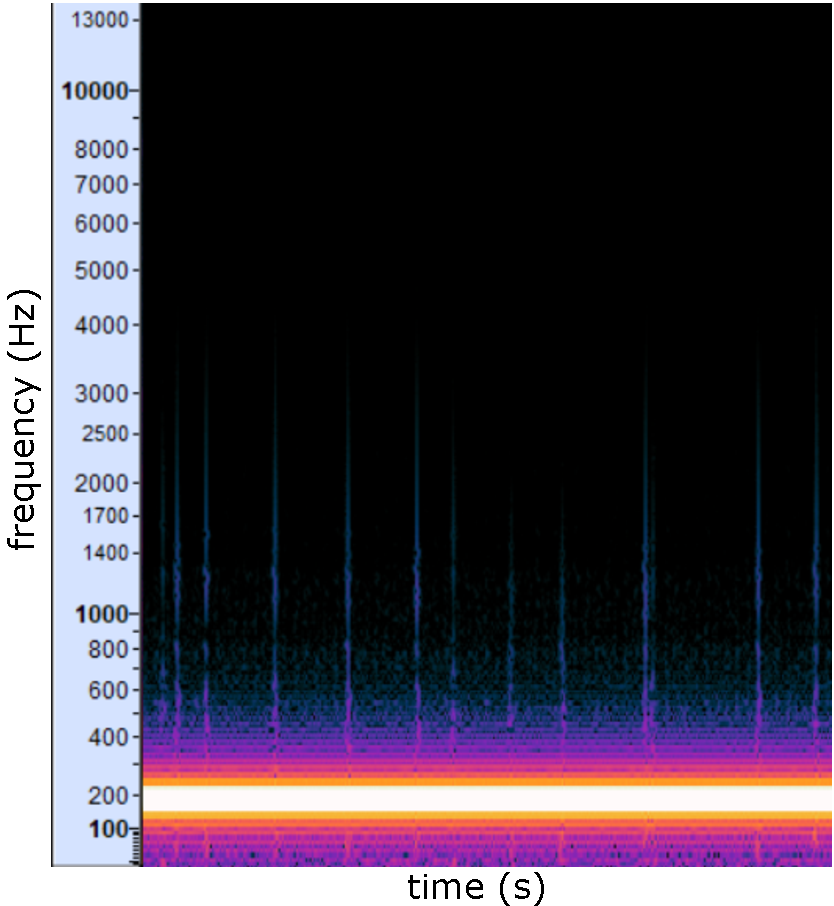
\includegraphics[width=0.9\linewidth]{Assets/Figures/Illustrations/G3_196Hz_PureTone_waveform_spectrogram.pdf}
					\caption{The frequency spectrogram of the audible waveform being a monotone and purely generated G3-tone at 195.99 Hz \cite{generate_tones}.}
					\label{fig:sub:G3_pure_waveform}
				\end{subfigure}%
				\begin{subfigure}[t]{.5\textwidth}
					\centering\captionsetup{width=.9\linewidth}%
					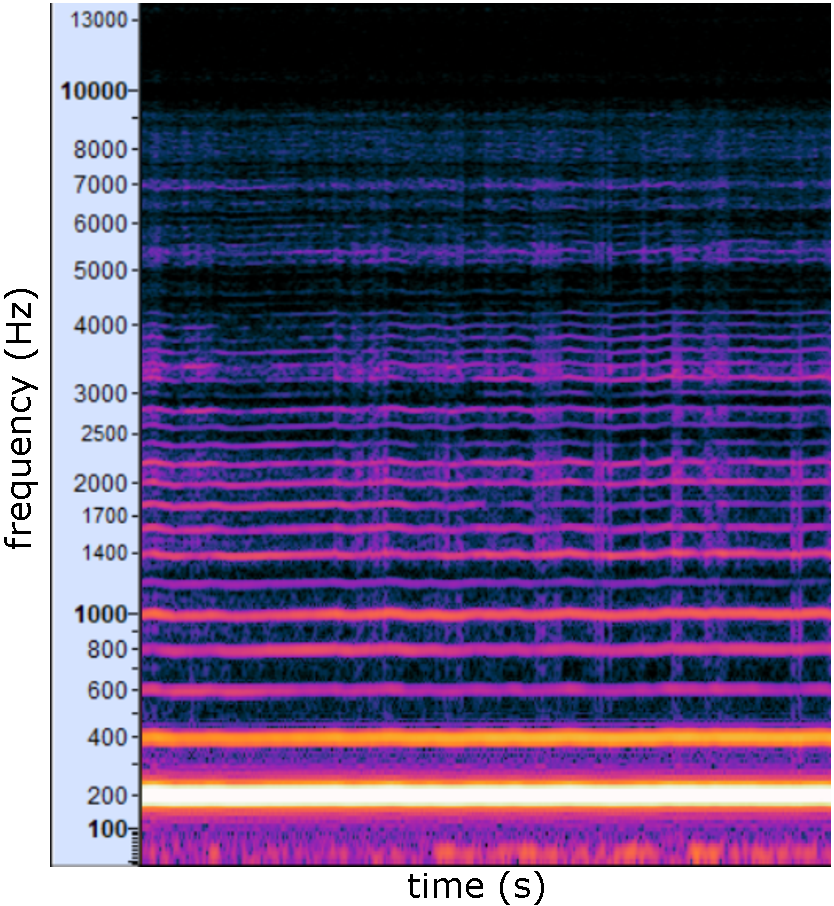
\includegraphics[width=0.9\linewidth]{Assets/Figures/Illustrations/G3_196Hz_HummingWaveform_FrequencySpectrum.pdf}
					\caption{The frequency spectrogram of the audible waveform being a more-or-less monotone but non-pure G3-tone, hummed and recorded by me \cite{}, as I tried to repeat the tone in \ref{fig:sub:G3_pure_waveform} with my voice.}
					\label{fig:sub:G3_hummed_waveform}
				\end{subfigure}
			\caption[Frequency spectrograms illustrating the absence and presence of harmonics and overtones in audible waveforms]{Frequency spectrograms of two different-sounding waveforms of the same G3-tone at 195.99 Hz. Note the absence and presence of harmonics and overtones in waveform \ref{fig:sub:G3_pure_waveform} and \ref{fig:sub:G3_hummed_waveform} respectively, as well as the integer-relationships between the fundamental (lowest) frequency and the harmonics in \ref{fig:sub:G3_hummed_waveform}. Frequencies in a harmonically synchronized agent collective will for the first $\phi$-problem resemble the frequencies in \ref{fig:sub:G3_pure_waveform}, where all frequencies are equal and constant. Conversely, when frequencies can be heterogenous and unequal, as in the $\phi$- \& $\omega$-problem, the frequencies in a harmonically synchronized agent collective will rather resemble the frequencies in \ref{fig:sub:G3_hummed_waveform}, where these higher frequencies with integer-relationships to the fundamental and lowest frequency can be present.}
			\label{fig:frequency_spectrograms}
		\end{figure}

		More accurately then, and inspired by integer-relationships in the frequencies of harmonics and the fundamental frequency in the spectrogram of a waveform, K. Nymoen et al. \cite{nymoen_synch} describe the \textit{legal} frequencies the robots's oscillators in the musical robot collective have to adhere to in order for the oscillator-frequencies to be considered \textit{harmonically synchronized}:

		All musical robots $i$, in a harmonically synchronized state, will have frequencies $\omega_i$ which are element in the mathematical set

		\begin{equation}\label{legal_freqs}
		\Omega_{legal}(\omega_0) = \omega_{0} \cdot 2^{\mathbb{N}_0} = \{\omega_{0}, 2\omega_{0}, 4\omega_{0}, 8\omega_{0}, ...\} ,
		\end{equation}

		where $\omega_{0}$ is the lowest frequency in the robot-collective (or the fundamental frequency if you will), and $\mathbb{N}_0$ are the natural numbers including the number zero. If e.g. the smallest oscillator-frequency in the musical robot collective ($\omega_0$) was equal to 1.5Hz, \textit{legal} oscillator-frequencies the rest of the musical robots in the collective could have would be $\Omega_{legal}$(1.5Hz) = \{1.5Hz, 3Hz, 6Hz, 12Hz, ...\}.

		Hence, in terms of oscillator-/robot-frequencies $\omega_i$ for all robots $i$, we have a harmonically synchronized robot-collective if (and only if)

		\begin{equation}\label{synced_freqs}
		\omega_i \in \Omega_{legal}(\omega_0) , \forall i ,
		\end{equation}

		where we then say all robots in the robot-collective have \textit{legal} frequencies.



		This state of \textit{harmonic synchrony} is then the system goal state K. Nymoen et al. achieve using their phase- and frequency-update/-adjustment functions, as explained above in Section 3.3 and 3.4, and is also the target/goal state we want to continue achieving in this thesis, but hopefully with even more \textit{self-aware} methods (which are hopefully quicker and more robust).


			\subsection{Detecting harmonic synchrony}
			\label{subsec:harmonic_synchrony}
			In order to test and evaluate synchronization-performance in their firefly-inspired oscillator-system, K. Nymoen et al. \cite{nymoen_synch} develop a measure used to detect when the system has reached a state of synchrony. Using the firings of the fireflies, some well-defined conditions have to be met in order for the fireflies to be deemed \textit{harmonically synchronized}:
			\begin{itemize}
				\item \textbf{Condition 1}: Firing may only happen within a short time-period $t_f$.
				\item \textbf{Condition 2}: All nodes must have fired at least once during the evaluation period.
				\item \textbf{Condition 3}: Between each $t_f$, a period $t_q$ without fire events must be equally long $k$ times in a row.
			\end{itemize}
			
			By utilizing transmitted firings/pulses from the robots in our robot-collective, these conditions can be enforced and checked throughout the synchronization-process, in order to detect if the oscillator-network becomes harmonically synchronized.
			
			For getting a better idea of how these conditions being met looks like, see the \textit{performance-measure plot} in Figure \ref{fig:perf_measure_plot} where the oscillators/robots fulfill the abovementioned requirements right before ending the synchronization process.
			
			These requirements, amongst other illustrations in Nymoen et al.'s paper \cite{nymoen_synch}, thus constitutes a blueprint for the design of a performance-/synchrony-measure able to detect the achievement of harmonic synchrony in a decentralized network of ``firing''—or pulse-coupled—oscillators. The time having passed from the start of the synchronization-process until the detection of harmonic synchrony will then be defined as the performance-score, indicating how fast or slow the oscillators are at synchronizing.
			
			The exact details of how such a performance-/synchrony-measure is implemented for our musical multi-robot oscillator-network, in the synchronization-simulator, will be given in Section \ref{sec:performance_measure}.
	
	
	\chapter{dubby-hack Tools n stuff}
	
	\chapter{Implementation}
	\label{chap:implementation}
	
		\section{Simulator setup: the musical multi-robot collective}
		\section{Synchronizing oscillator-phases}
		\section{Synchronizing oscillator-frequencies}
	
		\section{Performance-/synchrony-measure: detecting harmonic synchrony}
		\label{sec:performance_measure}

		The performance-measure will be used in our synchrony-simulator to evaluate and test the multi-robot collective's ability to harmonically synchronize to each other. As mentioned in Subsection \ref{subsec:harmonic_synchrony}, K. Nymoen et al.'s requirements and illustrations \cite{nymoen_synch} for achieving \textit{harmonic synchrony} serve as a blueprint or guide for how to similarly implement our synchrony-/performance-measure. This performance-measure should be able to, during synchronization-simulation, detect if harmonic synchronization has been achieved in our decentralized oscillator-network. The successful triggering of this detection will then in turn terminate the synchronization simulation-run and save to a dataset the time it took to synchronize (the performance-score), in the case of a `synchronization-success' — an example of which can be seen in Figure \ref{fig:perf_measure_plot}.

		\begin{figure}
			\centering
			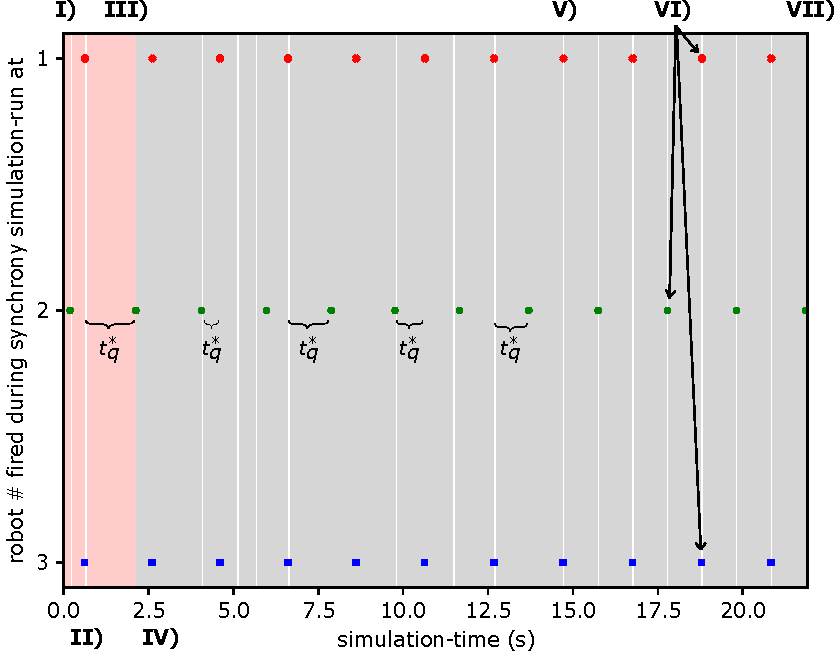
\includegraphics[width=\linewidth]{Assets/Figures/Illustrations/ExplanatoryIllustrativePerfMeasurePlot.pdf}
			\caption[A \textbf{performance-measure plot}.]{\textbf{Performance-/synchrony-measure plot}: recording a detection of harmonic synchrony. Initial red area represents the ``start-up''-period where no (gray) $t_q$-value is defined yet. \textbf{I)} First robot firing, initiating a process of defining such a ``silent'' time-window $t_q$ within which no nodes are allowed to fire, and a whole ``legal-firing'' $t_f$-window (here shaded in white and only 80ms long, as in \cite{nymoen_synch}) ensues. \textbf{II)} At least one robot firing, and with their firing-time(s) giving us the \textit{early $t_q$-defining} time-value (see schema below), as well as triggering second whole $t_f$-window to ensue. \textbf{III)} At least one robot firing after the \textit{early $t_q$-defining} time-value was found, hence (with their firing-time(s)) giving us the \textit{late $t_q$-defining} time-value right before using these when finishing the on-started process of defining the ``silent'' time-window $t_q$; triggering a half (due to stabilization purposes by future centering of fire-events) $t_f$-window to ensue. \textbf{IV)} A robot is caught firing illegally during a ``silent'' $t_q$-window and hence resets the \textit{towards\_k\_counter}-variable, as well as (re-) starts a process like in \textbf{I)} for (re-) defining a new $t_q$-value. \textbf{V)} Firing after this point only happens during short ``legal-firing'' $t_f$-windows, so \textbf{Condition 1} (cf. \ref{subsec:harmonic_synchrony}) is held. \textbf{VI)} All robots have fired at least once during the evaluation-period, so \textbf{Condition 2} is held. \textbf{VII)} The robot collective has fired legally and evenly, without resetting $t_q$, $k$ (equal to 8 in this case) times in a row, so \textbf{Condition 3} is fulfilled — and harmonic synchrony is thus achieved and detected after 21.9 seconds of synchronization.}
			\label{fig:perf_measure_plot}
		\end{figure}

		The resulting and corresponding performance-scores obtained using this perf-ormance-measure will then take values of the simulation-time (in seconds) it takes for the robot-collective, from the start of the synchronization-simulation, to achieve the system target state of \textit{harmonic synchrony}, as specified in Section \ref{sec:harmonic_synchrony}.

		Now if \textbf{Conditions 1-3} from Subsection \ref{subsec:harmonic_synchrony} are kept, we have harmonic synchrony.

		My specific implementation of the performance-/synchrony-measure essentially consists of enforcing all the requirements or rules listed in \ref{subsec:harmonic_synchrony}, given some constant $t_f$- and $k$-values (e.g. $80ms$ and $8$ respectively \cite{nymoen_synch}). And again—to recall from \ref{subsec:harmonic_synchrony}—$t_f$ is the short time-window within which nodes are allowed to fire at each beat, and $k$ represents how many times nodes have to fire at even underlying pulses/beats in a row without changing the $t_q$-period—before becoming harmonically synchronized.

		The requirement of firing evenly $k$ times in a row with identical $t_q$-periods can be—and in fact is in our implementation—enforced by incrementing an integer variable \textit{towards\_k\_counter} after a `legal' $t_f$-window has occured (i.e. one or more nodes fired inbetween the onset and ending of the $t_f$-window), and conversely by resetting \textit{towards\_k\_counter} to 0 when an illegally transmitted firing was heard during a `silent' (or so it was supposed to be at least) $t_q$-window, hence restarting the synchrony-detection process—as can be seen occuring several times in Figure \ref{fig:synch_evolution_perf_measure_ill}.

		\begin{figure}[h]
			\centering
			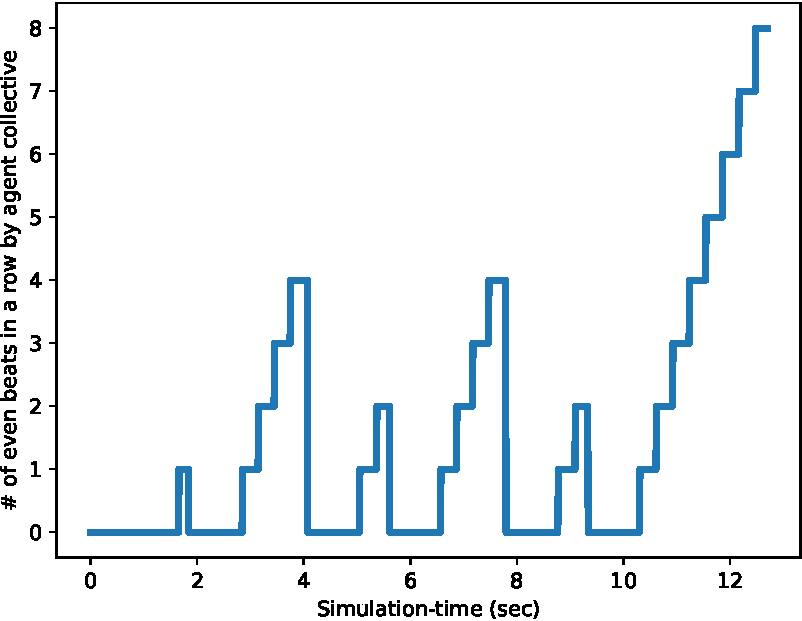
\includegraphics[width=0.85\linewidth]{Assets/Figures/Illustrations/SynchronyEvolutionPerfMeasureIllustration.pdf}
			\caption[A \textbf{synchrony-evolution plot}.]{A \textbf{synchrony-evolution plot}, displaying the temporal recording of the \textit{towards\_k\_counter}-variable throughout a synchrony simulation-run in Unity. The counter is incremented as the robot-collective fires evenly within `legal' $t_f$-windows, and is conversely reset to 0 if illegal firings during `silent' $t_q$-windows are heard. Note that in this specific simulation-run above, the agents were on their way to achieve harmonic synchrony five times before the 10th second of the synchronization-simulation already, but since one or more of them fired `illegally' (i.e. inside a $t_q$-window), they were consequently `punished'—or rather deemed `not synchronized enough yet'—by getting their counter reset to 0. Eventually however,  through further phase- \& frequency-synchronization, the multi-robot collective was in this case after 12.5 seconds able to achieve harmonic synchrony, when \textit{towards\_k\_counter} became equal to $k$, as well as all other requirements for achieving \textit{harmonic synchrony} was met.}
			\label{fig:synch_evolution_perf_measure_ill}
		\end{figure}

		Initially, the $t_q$-period/-window is not initialized, as it entirely depends on the frequencies to which the robot-collective converges to; however, when an illegal firing (i.e. a firing perceived during a $t_q$-window) occurs—$t_q$ is also then reset itself to a hopefully more correct value, given by the following formula, which is visually explained further in the schema in Figure \ref{fig:t_q_schema}:

		\begin{equation}
		\label{t_q_definition}
		\begin{array}{rrclcl}
		t_q^* & = & late\_t_q^*\_defining\_timevalue - early\_t_q^*\_defining\_timevalue - t_f \\
		& = & median(t_1^`, t_2^`, ..., t_m^`) - median(t_1, t_2, ..., t_n) - t_f , \\
		\end{array}
		\end{equation}

		where $n$ fire-events were recorded during the earlier $t_f$-window, and $m$ fire-events were recorded during the later $t_f$-window.


		\begin{figure}[ht!]
			\centering
			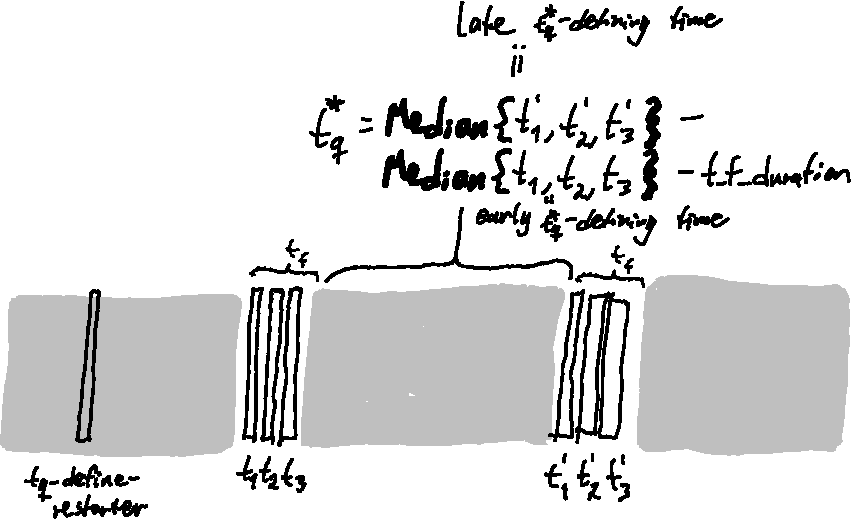
\includegraphics[width=0.85\linewidth]{Assets/Figures/Illustrations/t_q_schema.pdf}
			\caption{Schema: how ``silent'' $t_q$-windows are defined. \tcol[red]{Til Kyrre: Dette var bare grovt, som jeg tenker jeg må lage mer profesjonelt i Inkscape ellernoe.}}
			\label{fig:t_q_schema}
		\end{figure}


		The specific steps and procedures needed to implement this performance-/synchrony-measure is expounded in detail in Algorithms \ref{perf_synch_measure_algo_A}, \ref{perf_synch_measure_algo_B}, and \ref{perf_synch_measure_algo_C}.

		\begin{algorithm}
		\caption{Performance-/synchrony-measure part A \tcol[red]{(må evt. fylles inn)}}\label{perf_synch_measure_algo_A}
		\end{algorithm}

		\begin{algorithm}
		\caption{Performance-/synchrony-measure part B \tcol[red]{(må evt. fylles inn)}}\label{perf_synch_measure_algo_B}
		\end{algorithm}

		If a certain amount of time, e.g. 5 minutes \cite{nymoen_synch}, has gone without the detection of harmonic synchrony occuring, the simulation-run is terminated as a ``fail''.
	
	
		
	% Document Footer (Bibliography, Appendices etc.).
	\newpage

% Bibliography.
\printbibliography % VIL KALLE DEN 'References' ISTEDENFOR 'Bibliography'?

% Appendices (A, B, C, D, ...) {
	% A: Synonym-list w/explanations, if not managing to be consistent.
	% B: The Developed Code? Only GitHub-repo links?
	% C: Other secondary figures/plots.
% }
\end{document}